%% %% %% %%
%%
%% Parte C de la práctica
%%
%% %% %% %%

\documentclass[../procedimientos.tex]{subfiles}
\graphicspath{{\subfix{../../images/}}}

\begin{document}
\clearpage
\subsection{Parte C}
\subsubsection{Propuesta}
\paragraph{Nota.} Se utilizará el mismo problema propuesto en la clase pasada 
con la finalidad de implentarlo en VHDL.

\begin{em}
  Luis, Ana y sus padres van al cine bajo ciertas condiciones que son limitadas 
  por la Madre y el Padre.  Ellos van al cine si la Madre y el Padre están 
  totalmente de acuerdo, si los dos no lo están, entonces no pueden ir.  Ahora, 
  si los dos están en desacuerdo, la salida al cine debe ser resuelta por 
  mayoría absoluta entre todos los integrantes de la familia.  Si existe un 
  empate general, la decisión será tomada por la madre.  Diseñar un circuito 
  digital que señalice con un diodo LED el momento cuando pueden ir al cine.
\end{em}

\subsubsection{Análisis}
De forma general, el sistema tiene cuatro entradas: $l$, $a$, $m$ Y $p$ (el 
voto de Luis, Ana, su Madre y su Padre respectivamente); y la salida estará 
dada por el valor de $c(lamp)$.  La Implementación de la tabla de verdad del 
problema se muestra a continuación:
\begin{table}[H]
  \centering
  \begin{tabular}{cccc|ccc}
    \hline
    $l$ & $a$ & $m$ & $p$ & $c$\\
    \hline
    0 & 0 & 0 & 0 & 0\\
    0 & 0 & 0 & 1 & 0\\
    0 & 0 & 1 & 0 & 0\\
    0 & 0 & 1 & 1 & 1\\
    0 & 1 & 0 & 0 & 0\\
    0 & 1 & 0 & 1 & 0\\
    0 & 1 & 1 & 0 & 1\\
    0 & 1 & 1 & 1 & 1\\
    1 & 0 & 0 & 0 & 0\\
    1 & 0 & 0 & 1 & 0\\
    1 & 0 & 1 & 0 & 1\\
    1 & 0 & 1 & 1 & 1\\
    1 & 1 & 0 & 0 & 0\\
    1 & 1 & 0 & 1 & 1\\
    1 & 1 & 1 & 0 & 1\\
    1 & 1 & 1 & 1 & 1\\
    \hline
  \end{tabular}
  \caption{Tabla de verdad del problema (Sección C)}
  \label{tab:tv_c}
\end{table}

Con lo anterior, se puede deducir la forma canónica \textit{SOP}, tal como se 
muestra a continuación:
\begin{equation*}
  c(lamp) = \sum_m (3, 6, 7, 10, 11, 13, 14, 15)
\end{equation*}

La simplificación se llevará a cabo con ayuda del método de \textit{Mapas de 
Karnaugh}.
\begin{figure}[H]
  \centering
  \begin{karnaugh-map}[4][4][1][$p$][$m$][$a$][$l$]
    \minterms{3,6,7,10,11,13,14,15}
    \implicant{15}{10}
    \implicant{7}{14}
    \implicant{3}{11}
    \implicant{13}{15}
  \end{karnaugh-map}
\end{figure}

La lectura del mapa nos indica que:
\begin{equation*}
  c(lamp) = mp + am + lm + lap
\end{equation*}

Simplificando un poco la expresión, se tiene que:
\begin{equation*}
  \boxed{
    \therefore c(lamp) = m(p + a + l) + lap
  }
\end{equation*}

De forma general, lo anterior nos indica que si la Mamá quiere ir al cine y al 
menos alguien más también quiere ir, entonces irán al cine; la única otra 
forma de ir al cine es cuando tanto Luis, Ana y el Papá quieren ir.

\subsubsection{Implementación en Quartus}
Con la reducción anterior, se implementó el sistema dentro de la plataforma 
\textit{Quartus II}.  Para esto, después de crear el proyecto, se creó un 
nuevo archivo de tipo \textbf{VHDL}, el cual tiene el contenido mostrado a 
continuación:
\begin{lstlisting}[language=VHDL, caption=Archivo VHDL (Parte C)]
-- Implementacion: Parte C

library ieee;
use ieee.std_logic_1164.all;

entity p04c is
	port(
		l,a,m,p		:in	std_logic;
		c				:out	std_logic
	);
end;

architecture simple of p04c is
begin
	c <= (m and (l or a or p)) or (l and a and p);
end;
\end{lstlisting}

Con lo anteiror, se ejecutó una simulación funcional dentro de \textit{Quartus 
II}, con lo cual se obtuvieron las siguientes salidas:
\begin{figure}[H]
  \centering
  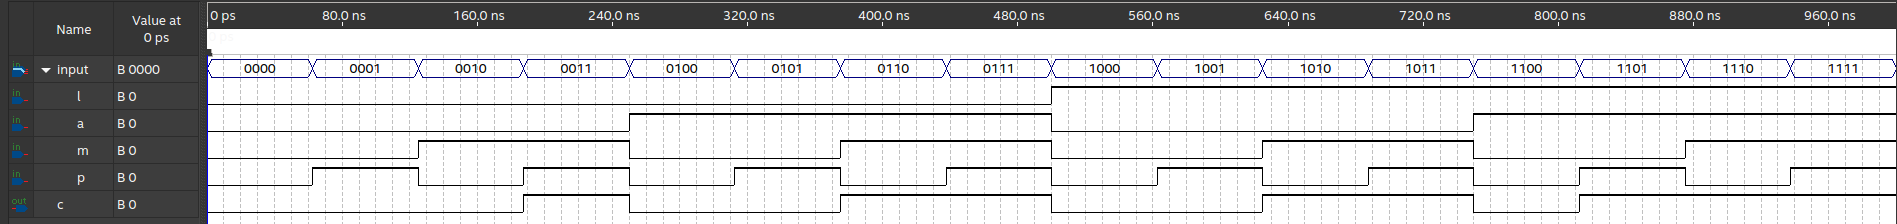
\includegraphics[width=\textwidth]{sim_c}
  \caption{Simulación Funcional (Parte C)}
\end{figure}

Esto coincide con los valores establecidos en la Tabla \ref{tab:tv_c}. Con lo 
cual, el sistema se implementó de forma adecuada.
\end{document}


